%%**************************************************************
%% Vorlage fuer Bachelorarbeiten (o.ä.) der DHBW
%%
%% Autor: Tobias Dreher, Yves Fischer
%% Datum: 06.07.2011
%%
%% Autor: Michael Gruben
%% Datum: 15.05.2013
%%
%% Autor: Markus Barthel
%% Datum: 22.08.2014
%%**************************************************************

%!TEX root = ../dokumentation.tex

%
% Nahezu alle Einstellungen koennen hier getaetigt werden
%

\RequirePackage[l2tabu, orthodox]{nag}	% weist in Commandozeile bzw. log auf veraltete LaTeX Syntax hin

\documentclass[%
	pdftex,
	oneside,			% Einseitiger Druck.
	12pt,				% Schriftgroesse
	parskip=half,		% Halbe Zeile Abstand zwischen Absätzen.
%	topmargin = 10pt,	% Abstand Seitenrand (Std:1in) zu Kopfzeile [laut log: unused]
	headheight = 12pt,	% Höhe der Kopfzeile
%	headsep = 30pt,	% Abstand zwischen Kopfzeile und Text Body  [laut log: unused]
	headsepline,		% Linie nach Kopfzeile.
	footsepline,		% Linie vor Fusszeile.
	footheight = 16pt,	% Höhe der Fusszeile
	abstracton,		% Abstract Überschriften
	DIV=calc,		% Satzspiegel berechnen
	BCOR=8mm,		% Bindekorrektur links: 8mm
	headinclude=false,	% Kopfzeile nicht in den Satzspiegel einbeziehen
	footinclude=false,	% Fußzeile nicht in den Satzspiegel einbeziehen
	listof=totoc,		% Abbildungs-/ Tabellenverzeichnis im Inhaltsverzeichnis darstellen
	toc=bibliography,	% Literaturverzeichnis im Inhaltsverzeichnis darstellen
]{scrreprt}	% Koma-Script report-Klasse, fuer laengere Bachelorarbeiten alternativ auch: scrbook

% Einstellungen laden
\usepackage{xstring}
\usepackage[utf8]{inputenc}
\usepackage[T1]{fontenc}

\newcommand{\einstellung}[1]{%
  \expandafter\newcommand\csname #1\endcsname{}
  \expandafter\newcommand\csname setze#1\endcsname[1]{\expandafter\renewcommand\csname#1\endcsname{##1}}
}
\newcommand{\langstr}[1]{\einstellung{lang#1}}

\einstellung{martrikelnr}
\einstellung{titel}
\einstellung{kurs}
\einstellung{datumAbgabe}
\einstellung{firma}
\einstellung{firmenort}
\einstellung{abgabeort}
\einstellung{abschluss}
\einstellung{studiengang}
\einstellung{dhbw}
\einstellung{betreuer}
\einstellung{gutachter}
\einstellung{zeitraum}
\einstellung{arbeit}
\einstellung{autor}
\einstellung{sprache}
\einstellung{schriftart}
\einstellung{seitenrand}
\einstellung{kapitelabstand}
\einstellung{spaltenabstand}
\einstellung{zeilenabstand}
\einstellung{zitierstil}
 % verfügbare Einstellungen
%%%%%%%%%%%%%%%%%%%%%%%%%%%%%%%%%%%%%%%%%%%%%%%%%%%%%%%%%%%%%%%%%%%%%%%%%%%%%%%
%                                   Einstellungen
%
% Hier können alle relevanten Einstellungen für diese Arbeit gesetzt werden.
% Dazu gehören Angaben u.a. über den Autor sowie Formatierungen.
%
%
%%%%%%%%%%%%%%%%%%%%%%%%%%%%%%%%%%%%%%%%%%%%%%%%%%%%%%%%%%%%%%%%%%%%%%%%%%%%%%%


%%%%%%%%%%%%%%%%%%%%%%%%%%%%%%%%%%%% Sprache %%%%%%%%%%%%%%%%%%%%%%%%%%%%%%%%%%%
%% Aktuell sind Deutsch und Englisch unterstützt.
%% Es werden nicht nur alle vom Dokument erzeugten Texte in
%% der entsprechenden Sprache angezeigt, sondern auch weitere
%% Aspekte angepasst, wie z.B. die Anführungszeichen und
%% Datumsformate.
\setzesprache{en} % oder en
%%%%%%%%%%%%%%%%%%%%%%%%%%%%%%%%%%%%%%%%%%%%%%%%%%%%%%%%%%%%%%%%%%%%%%%%%%%%%%%%

%%%%%%%%%%%%%%%%%%%%%%%%%%%%%%%%%%% Angaben  %%%%%%%%%%%%%%%%%%%%%%%%%%%%%%%%%%%
%% Die meisten der folgenden Daten werden auf dem
%% Deckblatt angezeigt, einige auch im weiteren Verlauf
%% des Dokuments.
\setzemartrikelnr{29015}
\setzekurs{}
\setzetitel{Simulating the GPU-based shaders in the graphics pipeline on a CPU-based language to allow code inspection at runtime}
%\setzetitel{Logfileanalyse mit Apache{\textsuperscript{TM}} Hadoop\textsuperscript{{\textregistered}} MapReduce}
\setzedatumAbgabe{September 2019}
\setzefirma{Firmenname}
\setzefirmenort{ORT}
\setzeabgabeort{Weingarten}
\setzeabschluss{nothing}
\setzestudiengang{nothing}
\setzedhbw{Ravensburg-Weingarten}
\setzebetreuer{Daniel Scherzer}
\setzegutachter{Sebastian Mauser}
\setzezeitraum{12 Wochen}
\setzearbeit{Masterthesis}
\setzeautor{Matthias Mettenleiter}
%%%%%%%%%%%%%%%%%%%%%%%%%%%%%%%%%%%%%%%%%%%%%%%%%%%%%%%%%%%%%%%%%%%%%%%%%%%%%%%%

%%%%%%%%%%%%%%%%%%%%%%%%%%%% Literaturverzeichnis %%%%%%%%%%%%%%%%%%%%%%%%%%%%%%
%% Bei Fehlern während der Verarbeitung bitte in ads/header.tex bei der
%% Einbindung des Pakets biblatex (ungefähr ab Zeile 110,
%% einmal für jede Sprache), biber in bibtex ändern.
\newcommand{\ladeliteratur}{%
\addbibresource{bibliographie.bib}
%\addbibresource{weitereDatei.bib}
}

\newcommand\myCite[1]{
	[\cite{#1}]
}
%% Zitierstil
%% siehe: http://ctan.mirrorcatalogs.com/macros/latex/contrib/biblatex/doc/biblatex.pdf (3.3.1 Citation Styles)
%% mögliche Werte z.B numeric-comp, alphabetic, authoryear
\setzezitierstil{authoryear}
%%%%%%%%%%%%%%%%%%%%%%%%%%%%%%%%%%%%%%%%%%%%%%%%%%%%%%%%%%%%%%%%%%%%%%%%%%%%%%%%

%%%%%%%%%%%%%%%%%%%%%%%%%%%%%%%%% Layout %%%%%%%%%%%%%%%%%%%%%%%%%%%%%%%%%%%%%%%
%% Verschiedene Schriftarten
% laut nag Warnung: palatino obsolete, use mathpazo, helvet (option scaled=.95), courier instead
\setzeschriftart{lmodern} % palatino oder goudysans, lmodern, libertine

%% Paket um Textteile drehen zu können
%\usepackage{rotating}
%% Paket um Seite im Querformat anzuzeigen
%\usepackage{lscape}

%% Seitenränder
\setzeseitenrand{2.5cm}

%% Abstand vor Kapitelüberschriften zum oberen Seitenrand
\setzekapitelabstand{20pt}

%% Spaltenabstand
\setzespaltenabstand{10pt}
%%Zeilenabstand innerhalb einer Tabelle
\setzezeilenabstand{1.5}
%%%%%%%%%%%%%%%%%%%%%%%%%%%%%%%%%%%%%%%%%%%%%%%%%%%%%%%%%%%%%%%%%%%%%%%%%%%%%%%%

%%%%%%%%%%%%%%%%%%%%%%%%%%%%% Verschiedenes  %%%%%%%%%%%%%%%%%%%%%%%%%%%%%%%%%%%
%% Farben (Angabe in HTML-Notation mit großen Buchstaben)
\newcommand{\ladefarben}{%
	\definecolor{LinkColor}{HTML}{00007A}
	\definecolor{ListingBackground}{HTML}{FCFAFB}
}
%% Mathematikpakete benutzen (Pakete aktivieren)
\usepackage{amsmath}
\usepackage{amssymb}

%% Programmiersprachen Highlighting (Listings)
\newcommand{\listingsettings}{%
	\lstset{%
		language=Java,			% Standardsprache des Quellcodes
		numbers=left,			% Zeilennummern links
		stepnumber=1,			% Jede Zeile nummerieren.
		numbersep=5pt,			% 5pt Abstand zum Quellcode
		numberstyle=\tiny,		% Zeichengrösse 'tiny' für die Nummern.
		breaklines=true,		% Zeilen umbrechen wenn notwendig.
		breakautoindent=true,	% Nach dem Zeilenumbruch Zeile einrücken.
		postbreak=\space,		% Bei Leerzeichen umbrechen.
		tabsize=2,				% Tabulatorgrösse 2
		basicstyle=\ttfamily\footnotesize, % Nichtproportionale Schrift, klein für den Quellcode
		showspaces=false,		% Leerzeichen nicht anzeigen.
		showstringspaces=false,	% Leerzeichen auch in Strings ('') nicht anzeigen.
		extendedchars=true,		% Alle Zeichen vom Latin1 Zeichensatz anzeigen.
		captionpos=b,			% sets the caption-position to bottom
		backgroundcolor=\color{ListingBackground}, % Hintergrundfarbe des Quellcodes setzen.
		xleftmargin=0pt,		% Rand links
		xrightmargin=0pt,		% Rand rechts
		frame=single,			% Rahmen an
		frameround=ffff,
		rulecolor=\color{darkgray},	% Rahmenfarbe
		fillcolor=\color{ListingBackground},
		keywordstyle=\color[rgb]{0.133,0.133,0.6}\bfseries,
		commentstyle=\color{Sepia},
		stringstyle=\color{red}
	}
}
%%%%%%%%%%%%%%%%%%%%%%%%%%%%%%%%%%%%%%%%%%%%%%%%%%%%%%%%%%%%%%%%%%%%%%%%%%%%%%%%

%%%%%%%%%%%%%%%%%%%%%%%%%%%%%%%% Eigenes %%%%%%%%%%%%%%%%%%%%%%%%%%%%%%%%%%%%%%%
%% Hier können Ergänzungen zur Präambel vorgenommen werden (eigene Pakete, Einstellungen)

% xcolor muss mit optionen vor pdfpages geladen werden
\usepackage[usenames,dvipsnames,table,xcdraw]{xcolor} 	%xcolor für HTML-Notation

\usepackage{pdfpages}
 % lese Einstellungen

\newcommand{\iflang}[2]{%
  \IfStrEq{\sprache}{#1}{#2}{}
}

\langstr{abkverz}
\langstr{anhang}
\langstr{glossar}
\langstr{deckblattabschlusshinleitung}
\langstr{artikelstudiengang}
\langstr{studiengang}
\langstr{anderdh}
\langstr{von}
\langstr{dbbearbeitungszeit}
\langstr{dbmatriknr}
\langstr{dbkurs}
\langstr{dbfirma}
\langstr{dbbetreuer}
\langstr{dbgutachter}
\langstr{sperrvermerk}
\langstr{erklaerung}
\langstr{abstract}
\langstr{listingname}
\langstr{listlistingname}
\langstr{listingautorefname}
 % verfügbare Strings
\input{lang/\sprache} % Übersetzung einlesen

% Einstellung der Sprache des Paketes Babel und der Verzeichnisüberschriften
\iflang{de}{\usepackage[english, ngerman]{babel}}
\iflang{en}{\usepackage[ngerman, english]{babel}} 


%%%%%%% Package Includes %%%%%%%

\usepackage[margin=\seitenrand,foot=1cm]{geometry}	% Seitenränder und Abstände
\usepackage[activate]{microtype} %Zeilenumbruch und mehr
\usepackage[onehalfspacing]{setspace}
\usepackage{makeidx}
\usepackage[autostyle=true,german=quotes]{csquotes}
\usepackage{tabularx}
\usepackage{longtable}
\usepackage{multirow}
\usepackage{enumitem}	% mehr Optionen bei Aufzählungen
\usepackage{graphicx}
%\usepackage[usenames,dvipsnames,table,xcdraw]{xcolor} 	%xcolor für HTML-Notation
\usepackage{float}
\usepackage{array}
\usepackage{calc}		% zum Rechnen (Bildtabelle in Deckblatt)
\usepackage[right]{eurosym}
\usepackage{wrapfig}
\usepackage{pgffor} % für automatische Kapiteldateieinbindung
\usepackage[perpage, hang, multiple, stable]{footmisc} % Fussnoten
%\usepackage[nohyperlinks]{acronym} % falls gewünscht kann die Option footnote eingefügt werden, dann wird die Erklärung nicht inline sondern in einer Fußnote dargestellt
\usepackage{acronym}

\usepackage{listings}

% Eigene zusätzliche packages
\usepackage{xfrac}
\usepackage{tikz}
\usepackage{subcaption}
%\usepackage[leqno]{amsmath}
%\usepackage{remreset}

% Wurzel mit schießendem Strich am ende
% New definition of square root: % it renames \sqrt as \oldsqrt
\let\oldsqrt\sqrt % it defines the new \sqrt in terms of the old one 
\def\sqrt{\mathpalette\DHLhksqrt} \def\DHLhksqrt#1#2{
\setbox0=\hbox{$#1\oldsqrt{#2\,}$}\dimen0=\ht0 \advance\dimen0-0.2\ht0 \setbox2=\hbox{\vrule height\ht0 depth -\dimen0}{\box0\lower0.4pt\box2}}

%\makeatletter
%\@removefromreset{equation}{chapter}
%\makeatother
%\renewcommand*{\theequation}{\arabic{equation}}

% eine Kommentarumgebung "k" (Handhabe mit \begin{k}<Kommentartext>\end{k},
% Kommentare werden rot gedruckt). Wird \% vor excludecomment{k} entfernt,
% werden keine Kommentare mehr gedruckt.
\usepackage{comment}
\specialcomment{k}{\begingroup\color{red}}{\endgroup}
%\excludecomment{k}


%%%%%% Configuration %%%%%

%% Anwenden der Einstellungen

\usepackage{\schriftart}
\ladefarben{}

% Titel, Autor und Datum
\title{\titel}
\author{\autor}
\date{\datum}

% PDF Einstellungen
\usepackage[%
	pdftitle={\titel},
	pdfauthor={\autor},
	pdfsubject={\arbeit},
	pdfcreator={pdflatex, LaTeX with KOMA-Script},
	pdfpagemode=UseOutlines, 		% Beim Oeffnen Inhaltsverzeichnis anzeigen
	pdfdisplaydoctitle=true, 		% Dokumenttitel statt Dateiname anzeigen.
	pdflang={\sprache}, 			% Sprache des Dokuments.
]{hyperref}

% (Farb-)einstellungen für die Links im PDF
\hypersetup{%
	colorlinks=true, 		% Aktivieren von farbigen Links im Dokument
	linkcolor=LinkColor, 	% Farbe festlegen
	citecolor=LinkColor,
	filecolor=LinkColor,
	menucolor=LinkColor,
	urlcolor=LinkColor,
	linktocpage=true, 		% Nicht der Text sondern die Seitenzahlen in Verzeichnissen klickbar
	bookmarksnumbered=true 	% Überschriftsnummerierung im PDF Inhalt anzeigen.
}
% Workaround um Fehler in Hyperref, muss hier stehen bleiben
\usepackage{bookmark} %nur ein latex-Durchlauf für die Aktualisierung von Verzeichnissen nötig

% Schriftart in Captions etwas kleiner
\addtokomafont{caption}{\small}

% Literaturverweise (sowohl deutsch als auch englisch)
\iflang{de}{%
\usepackage[
	backend=bibtex,		% empfohlen. Falls biber Probleme macht: bibtex
	bibwarn=true,
	bibencoding=utf8,	% wenn .bib in utf8, sonst ascii
	sortlocale=de_DE,
	style=\zitierstil,
	backref=true
]{biblatex}
}
\iflang{en}{%
\usepackage[
	backend=bibtex,		% empfohlen. Falls biber Probleme macht: bibtex
	bibwarn=true,
	bibencoding=utf8,	% wenn .bib in utf8, sonst ascii
	sortlocale=en_US,
	style=\zitierstil
]{biblatex}
}


% Mehr Platz zwischen einzelnen Items im Literaturverzeichnis bei Verwendung von authoryear
\setlength{\bibitemsep}{\baselineskip}
\DeclareNameAlias{sortname}{last-first}

\ladeliteratur{}

% Glossar
\usepackage[nonumberlist,toc]{glossaries}

%%%%%% Additional settings %%%%%%

% Hurenkinder und Schusterjungen verhindern
% http://projekte.dante.de/DanteFAQ/Silbentrennung
\clubpenalty = 10000 % schließt Schusterjungen aus (Seitenumbruch nach der ersten Zeile eines neuen Absatzes)
\widowpenalty = 10000 % schließt Hurenkinder aus (die letzte Zeile eines Absatzes steht auf einer neuen Seite)
\displaywidowpenalty=10000

% Bildpfad
\graphicspath{{images/}}

% Einige häufig verwendete Sprachen
\lstloadlanguages{PHP,Python,Java,C,C++,bash,XML}
\listingsettings{}
% Umbennung des Listings
\renewcommand\lstlistingname{\langlistingname}
\renewcommand\lstlistlistingname{\langlistlistingname}
\def\lstlistingautorefname{\langlistingautorefname}

% Umlaute ermöglichen in listings
\lstset{literate=
	{á}{{\'a}}1 {é}{{\'e}}1 {í}{{\'i}}1 {ó}{{\'o}}1 {ú}{{\'u}}1
	{Á}{{\'A}}1 {É}{{\'E}}1 {Í}{{\'I}}1 {Ó}{{\'O}}1 {Ú}{{\'U}}1
	{à}{{\`a}}1 {è}{{\`e}}1 {ì}{{\`i}}1 {ò}{{\`o}}1 {ù}{{\`u}}1
	{À}{{\`A}}1 {È}{{\'E}}1 {Ì}{{\`I}}1 {Ò}{{\`O}}1 {Ù}{{\`U}}1
	{ä}{{\"a}}1 {ë}{{\"e}}1 {ï}{{\"i}}1 {ö}{{\"o}}1 {ü}{{\"u}}1
	{Ä}{{\"A}}1 {Ë}{{\"E}}1 {Ï}{{\"I}}1 {Ö}{{\"O}}1 {Ü}{{\"U}}1
	{â}{{\^a}}1 {ê}{{\^e}}1 {î}{{\^i}}1 {ô}{{\^o}}1 {û}{{\^u}}1
	{Â}{{\^A}}1 {Ê}{{\^E}}1 {Î}{{\^I}}1 {Ô}{{\^O}}1 {Û}{{\^U}}1
	{œ}{{\oe}}1 {Œ}{{\OE}}1 {æ}{{\ae}}1 {Æ}{{\AE}}1 {ß}{{\ss}}1
	{ç}{{\c c}}1 {Ç}{{\c C}}1 {ø}{{\o}}1 {å}{{\r a}}1 {Å}{{\r A}}1
	{€}{{\EUR}}1 {£}{{\pounds}}1
}

% Weitere Keyword Highlights
\lstset{
	emph=[1]{ 
	    mkdir, jps, sudo, wget, mv, chown, su, adduser, addgroup, grep, sort, print, max, WARNING
    },
    emphstyle=[1]{\color[rgb]{0.133,0.133,0.6}},
    emph=[2]{
	    LFAConfiguration, Driver, Set, Exception, Configuration, FileInputFormat, FileOutputFormat, Job, Path, Text, IntWritable, Mapper, Matcher, Pattern, PatternMapper, Logger, Level, Context, IOException, InterruptedException, Reducer, CountReducer, TextInputFormat, TextOutputFormat, RecordReader, PDFInputFormat, PDFLineRecordReader, InputSplit, TaskAttemptContext, JobContext, CharSequence
    },
    emphstyle=[2]{\color[HTML]{006400}},
    emph=[3]{
	    String, int, Object, Iterable, boolean, Class, float
    },
    emphstyle=[3]{\color{Mulberry}}
}

% Abstände in Tabellen
\setlength{\tabcolsep}{\spaltenabstand}
\renewcommand{\arraystretch}{\zeilenabstand}


\makeglossaries
%!TEX root = ../dokumentation.tex

%
% vorher in Konsole folgendes aufrufen:
%	makeglossaries makeglossaries dokumentation.acn && makeglossaries dokumentation.glo
%

%
% Glossareintraege --> referenz, name, beschreibung
% Aufruf mit \gls{...}
%
\newglossaryentry{Glossareintrag}{name={Glossareintrag},plural={Glossareinträge},description={Ein Glossar beschreibt verschiedenste Dinge in kurzen Worten}}

\newglossaryentry{Commodity-Hardware}{name={Commodity-Hardware},description={\flqq Computer hardware that is affordable and easy to obtain. Typically it is a low-performance system that is IBM PC-compatible and is capable of running Microsoft Windows, Linux, or MS-DOS without requiring any special devices or equipment.\frqq\footcite{Beal.2015}}}

\newglossaryentry{Git}{name={Git},plural={Git},description={Git ist ein kostenloses System zur Versionskontrolle für kleine wie auch sehr große Projekte. ({\url{http://git-scm.com/}})}}

\newglossaryentry{NetBeans}{name={NetBeans},plural={NetBeans},description={The Smarter and Faster Way to Code Quickly and easily develop desktop, mobile and web applications with Java, HTML5, PHP, C/C++ and more. NetBeans IDE is FREE, open source, and has a worldwide community of users and developers. ({\url{https://netbeans.org}})}}

\newglossaryentry{Maven}{name={Maven},plural={Maven},description={Apache Maven is a software project management and comprehension tool. Based on the concept of a project object model (POM), Maven can manage a project’s build, reporting and documentation from a central piece of information. \\ ({\url{http://maven.apache.org/}})}}

\newglossaryentry{Nagios}{name={Nagios},plural={Nagios},description={Nagios Is The Industry Standard In IT Infrastructure Monitoring. Achieve instant awareness of IT infrastructure problems, so downtime doesn't adversely affect your business. Nagios offers complete monitoring and alerting for servers, switches, applications, and services. \\ ({\url{https://www.nagios.org}})}}

\newglossaryentry{Zabbix}{name={Zabbix},plural={Zabbix},description={Zabbix is the ultimate enterprise-level software designed for real-time monitoring of millions of metrics collected from tens of thousands of servers, virtual machines and network devices. Zabbix is Open Source and comes at no cost. \\ ({\url{http://www.zabbix.com}})}}

\newglossaryentry{Bootstrapping}{name={Bootstrapping},description={\flqq The computer term bootstrap began as a metaphor in the 1950s. In computers, pressing a bootstrap button caused a hardwired program to read a bootstrap program from an input unit. The computer would then execute the bootstrap program, which caused it to read more program instructions. It became a self-sustaining process that proceeded without external help from manually entered instructions. As a computing term, bootstrap has been used since at least 1953.\frqq\footcite[S. 1273]{Buchholz.1953}}}

\newglossaryentry{Generic}{name={Generic},plural={Generics},description={Ein Interface oder eine Klasse kann mit einem oder mehreren Parametern, den sog. Generics, definiert werden, welche zusätzliche Typangaben enthalten. Diese werden in spitzen Klammern notiert. Generics führen implizit einen Typumwandlung durch, welcher ohne Generics explizit erfolgen müsste\footcite[Vgl.][S. 4 f.]{Naftalin.2006}}}

\newglossaryentry{Plugin}{name={Plugin},plural={Plugins},description={\flqq Zusatzprogramm, welches über eine vordefinierte Schnittstelle in ein Basisprogramm eingebunden wird und dessen Funktionsumfang erweitert. [...] [Stammen] oftmals von anderen Herstellern als das Basisprogramm. [...] Plug-ins sind oft aus eigenständigen Programmen entstanden und können deshalb [...] i.d.R. auch ohne das Basisprogramm verwendet werden\frqq\footcite[]{Lackes.2015}}}

\begin{document}

	% Deckblatt
	\begin{spacing}{1}
		%!TEX root = ../dokumentation.tex

\begin{titlepage}
	\begin{longtable}{p{8.2cm} p{5.4cm}}
		{\raisebox{\ht\strutbox-\totalheight}{
\includegraphics[height=3.5cm]{images/rwu_logo_hor-lila-cyan_rgb.png}}} &
		{\raisebox{\ht\strutbox-\totalheight}{
\includegraphics[scale=0]{images/rwu_logo_hor-lila-cyan_rgb.png}}}
	\end{longtable}
	\enlargethispage{20mm}
	\begin{center}
		\vspace*{12mm}	{\LARGE\textbf \titel }\\
		\vspace*{12mm}
		\vspace*{12mm}	{\large\textbf \arbeit}\\
		%\vspace*{12mm}	\langdeckblattabschlusshinleitung\\
		\vspace*{12mm}
		%\vspace*{3mm}		{\textbf \abschluss}\\
		%\vspace*{12mm}	\langartikelstudiengang{} \langstudiengang{} \studiengang\\
    \vspace*{3mm}		\langanderdh{} \dhbw\\
		\vspace*{12mm}	\langvon\\
		\vspace*{3mm}		{\large\textbf \autor}\\
		\vspace*{12mm}	\datumAbgabe\\
	\end{center}
	\vfill
	\begin{spacing}{1.2}
	\begin{tabbing}
		mmmmmmmmmmmmmmmmmmmmmmmmmm             \= \kill
		\textbf{\langdbmatriknr}  \>  \martrikelnr\\
		\textbf{\langdbbetreuer}               \>  \betreuer\\
		\textbf{\langdbgutachter}              \>  \gutachter
	\end{tabbing}
	\end{spacing}
\end{titlepage}

	\end{spacing}
	\newpage

	% Sperrvermerk
%	%!TEX root = ../dokumentation.tex

\thispagestyle{empty}
% Sperrvermerk direkt hinter Titelseite
\section*{\langsperrvermerk}

\vspace*{2em}

\iflang{de}{%
  Die vorliegende {\arbeit} mit dem Titel {\itshape{} Logfileanalyse mit Apache\textsuperscript{\texttrademark} Hadoop\textsuperscript{\textregistered} MapReduce{}\/} enthält unternehmensinterne bzw. vertrauliche Informationen der {\firma}, ist deshalb mit einem Sperrvermerk versehen und wird ausschließlich zu Prüfungszwecken am Studiengang {\studiengang} der Dualen Hochschule Baden-Württemberg {\dhbw} vorgelegt. Sie ist ausschließlich zur Einsicht durch den zugeteilten Gutachter, die Leitung des Studiengangs und ggf. den Prüfungsausschuss des Studiengangs bestimmt.  Es ist untersagt,
  \begin{itemize}
  \item den Inhalt dieser Arbeit (einschließlich Daten, Abbildungen, Tabellen, Zeichnungen usw.) als Ganzes oder auszugsweise weiterzugeben,
  \item Kopien oder Abschriften dieser Arbeit (einschließlich Daten, Abbildungen, Tabellen, Zeichnungen usw.) als Ganzes oder in Auszügen anzufertigen,
  \item diese Arbeit zu veröffentlichen bzw. digital, elektronisch oder virtuell zur Verfügung zu stellen. 
  \end{itemize}
Jede anderweitige Einsichtnahme und Veröffentlichung – auch von Teilen der Arbeit – bedarf der vorherigen Zustimmung durch den Verfasser und {\firma}.
}

%http://www.ib.dhbw-mannheim.de/fileadmin/ms/bwl-ib/Downloads_alt/Leitfaden_31.05.pdf

\iflang{en}{%
  The {\arbeit} on hand 
  \begin{center}{\itshape{} Logfileanalyse mit Apache{\textsuperscript{TM}} Hadoop\textsuperscript{{\textregistered}} MapReduce{}\/}\end{center} 
   contains internal resp.\ confidential data of {\firma}. It is intended solely for inspection by the assigned examiner, the head of the {\studiengang} department and, if necessary, the Audit Committee \langanderdh{} {\dhbw}. It is strictly forbidden
    \begin{itemize}
    \item to distribute the content of this paper (including data, figures, tables, charts etc.) as a whole or in extracts,
    \item to make copies or transcripts of this paper or of parts of it,
    \item to display this paper or make it available in digital, electronic or virtual form.
    \end{itemize}
  Exceptional cases may be considered through permission granted in written form by the author and {\firma}.
}

\vspace{3em}

\abgabeort, \datumAbgabe
\vspace{4em}

\rule{6cm}{0.4pt}\\
\autor

%	\newpage

	% Erklärung
	%!TEX root = ../dokumentation.tex

\thispagestyle{empty}

\section*{\langerklaerung}
% http://www.se.dhbw-mannheim.de/fileadmin/ms/wi/dl_swm/dhbw-ma-wi-organisation-bewertung-bachelorarbeit-v2-00.pdf
\vspace*{2em}

\iflang{de}{%
Ich erkläre hiermit ehrenwörtlich: \\
\begin{enumerate}
\item dass ich meine {\arbeit} mit dem Thema
{\itshape \titel} ohne fremde Hilfe angefertigt habe;
\item dass ich die Übernahme wörtlicher Zitate aus der Literatur sowie die Verwendung der Gedanken
anderer Autoren an den entsprechenden Stellen innerhalb der Arbeit gekennzeichnet habe;
\item dass ich meine {\arbeit} bei keiner anderen Prüfung vorgelegt habe;
\item dass die eingereichte elektronische Fassung exakt mit der eingereichten schriftlichen Fassung
übereinstimmt.
\end{enumerate}

Ich bin mir bewusst, dass eine falsche Erklärung rechtliche Folgen haben wird.
}

% http://www.ib.dhbw-mannheim.de/fileadmin/ms/bwl-ib/Downloads_alt/Leitfaden_31.05.pdf (S. 52)

\iflang{en}{%
Hereby I solemnly declare:
\begin{enumerate}
\item that this {\arbeit}, titled {\itshape \title} is entirely the product of my own scholarly work, unless otherwise indicated in the text or references, or acknowledged below;
\item I have indicated the thoughts adopted directly or indirectly from other sources at the appropriate places within the document;
\item this {\arbeit} has not been submitted either in whole or part, for a degree at this or any other university or institution;
\item I have not published this {\arbeit} in the past; 
\item the printed version is equivalent to the submitted electronic one.
\end{enumerate}
I am aware that a dishonest declaration will entail legal consequences.
}

\vspace{3em}

\abgabeort, \datumAbgabe
\vspace{4em}

\rule{6cm}{0.4pt}\\
\autor

	\newpage

	% Abstract
	%!TEX root = ../dokumentation.tex

\pagestyle{empty}

\begin{abstract}

Debugging is an important part of the programming process. Most programming languages are supported by different debugging tools. For writing shaders within the graphics pipeline, the existing tools and support for debugging are scarce and most of the tools provided are limited to use with specific hardware and specific drivers for said hardware.

This thesis provides a solution to enable the use of different debugging tools for shaders in the graphics pipeline without the dependency on specific hardware or drivers while still providing the advantage of being executable on the GPU. To achieve this, the shader is written in a language supported by debugging tools while being executed in a simulated version of the graphics pipeline on the CPU. This shader is then translated to a regular shader language to run on the GPU.

\end{abstract}
	\newpage

	\pagestyle{plain}		% nur Seitenzahlen im Fuß
	
	%\RedeclareSectionCommand[beforeskip=\kapitelabstand]{chapter} % stellt Abstand vor Kapitelüberschriften ein

	% Inhaltsverzeichnis
	\begin{spacing}{1.1}
		\begingroup
		
			% auskommentieren für Seitenzahlen unter Inhaltsverzeichnis
			\renewcommand*{\chapterpagestyle}{empty}
			\pagestyle{empty}
			
			%\setcounter{tocdepth}{1}
			%für die Anzeige von Unterkapiteln im Inhaltsverzeichnis
			\setcounter{tocdepth}{2}
			
			\tableofcontents
			\clearpage
		\endgroup
	\end{spacing}
	\newpage
	
	\pagenumbering{Roman}

	
%	\newpage\null\thispagestyle{plain}\newpage


	\pagenumbering{arabic}
	
	\pagestyle{headings}		% Kolumnentitel im Kopf, Seitenzahlen im Fuß

	% Einleitung
	%!TEX root = ../dokumentation.tex

\chapter{Introduction}\label{cha:Introduction}

\paragraph{Explanation of debugging}

\paragraph{Problem with debugging of shaders in the graphics pipeline}

\paragraph{Existing approach for compute shaders}

\paragraph{Objective of creating a general solution for debuging shaders in the graphics pipeline}
	
	% Theoretische Grundlagen
	%!TEX root = ../dokumentation.tex

\chapter{Related Work}\label{cha:RelatedWork}
\section{Existing methods for debugging shaders in the graphics pipeline}
\label{section:debuggingMethods}

For debugging a shader program within the graphics pipeline there are the options to use workarounds to get the values of the variables within the code or to use special drivers provided by the producers of the hardware to get the option to debug on this hardware.

\paragraph{Manual debugging}

The manual way of debugging a shader is by creating outputs of the values within the shader program to see anomalies in their values. This can't be done by writing these values on the console or in a log file like it would be done in a CPU based application because as mentioned in \autoref{section:problems} there is no access to the console or a logger within a shader program. The workaround used here is to return the values projected on the rgba-color values on the resulting image of the program. In this way the programmer can see the rough area in which the values are located on the direct output. The image can also be saved and inspected closer to get the exact values within the pixels of the resulting image.\myCite{Ciardi.2015}

\paragraph{Debugging with special drivers on certain hardware}
\label{section:debuggingMethods_drivers}

It is possible to install special drivers for certain graphics cards provided by their producers to enable debugging of shaders running on this hardware within dedicated environments. The two big suppliers of graphics hardware Nvida and AMD provide these debugging environments in the form of \cite{Nvidia_Nsight} and \cite{AMD_GPUPerfStudio}. These tools can be included into different IDEs or downloaded as standalone applications. There are debugging tools for GPU debugging provided by other sources than the producers of the hardware themselves but for gaining access to the values in the hardware pipeline the drivers of this hardware have to implement specific debugging interfaces.\myCite{Microsoft_debug.2016} Applying these tools enables the use of breakpoints and the inspection of variables within the shader code at runtime\myCite{GLSL_debugger} or dumping the buffer into a file.\myCite{Microsoft_pdb.2019} The disadvantage of this method is that not all graphics cards are supported with such drivers and tools by their producer.

\section{Approaches for debugging compute shaders on the CPU}
\label{section:computeApproaches}

As \myCite{Jukka.2012} states "Relatively little has been published about debugging of GPU programs  in  practice.  Most  of  the  best  practice  guides  and lessons learned papers discuss GPU programming rather than debugging. Although exceptions exist". Among these exceptions are approaches to write compute shaders in other programming languages. The version of the shader in the other language can be run on the CPU where it can be debugged. This version of the shader will then be translated to the actual shader language so it can run on the GPU with the full performance advantage. This enables the use of all tools the chosen language supports to aid debugging without depending on specific hardware or drivers.
Examples implementing this for simulating CUDA shders in C\# are \myCite{ILGPU} and \myCite{Campy}.

The advantage compute shaders have in comparison with other kinds of shader programs is that they run independently of the graphics pipeline. For a compute shader a buffer of input data is defined. The compute shader is then executed writing the results in an output buffer. The output can be accessed by copying this buffer. This process can be emulated within a program running on the CPU by applying the calculations of this shader to the data as a function.

In comparison, for a shader in the graphics pipeline the inputs and outputs are handeled by the pipeline. The user defines the input for the pipeline itself. The shaders define how the data is processed within their corresponding stage and which data flows in and out of this stage. Inbetween the shader stages there are calculations applied to the data flowing through. These calculations are given by the pipeline. Here the individual shaders are dependent on the pipeline and the shaders for the other shader stages. Because of this emulating shaders in the graphics pipeline is more complex than emulating compute shaders.

\section{Translating shaders from other languages}\label{section:translating}

To run code on the GPU usually the programmer has to use one of  multiple low-level languages specialized in this task. To enable programmers to run code on the GPU while being able to stay at the language they are accustomed to there are multiple solutions to translate different languages into these low-level languages.

There are three different types of programming languages. The ones that are directly compiled ahead of time (AOT), the ones that are compiled to an intermediate language which then runs in a JIT(Just in Time) compiler and the ones that are running in an interpreter. For these three types there are different approaches to translate them to a shader language.\myCite{Turton.2017}

For all of these kinds of languages, it is possible to write a compiler translating them directly to the shader language. This is what \myCite{GLSLplusplus} does with the AOT compiled language C++ translating it to the shader language GLSL. In this project created to change the way of writing shader code the possibility of using this to debug the shaders written in C++ is mentioned. \myCite{SharpShader} is another example which uses the Language C\# which is usually compiled to the intermediate language MSIL. In this example C\# code is directly compiled to a Shader languages HLSL or GLSL. In both cases the programmer can use his accustomed language with the limitation of having to write the code for the GPU within special syntax rules to be able to translate it to be translated into a shader for the GPU. An advantage that results of the direct translation is that variable names given in the written code can be directly retained in the shader code.

Another option with the use of a language that compiles to an intermediate language is to take the code in the intermediate language and further translate it into a shader language. Examples implementing this are \myCite{ILGPU} and \myCite{Campy} where the shaders are written in C\#. This code is then compiled to the intermediate language MSIL. The MSIL code is further translated into the compute language CUDA which then runs on the GPU. Another example is \myCite{SpirvNet} which translates MSIL to Spirv. Spirv is a intermediate language for graphical shader code that can be interpreted as a shader on the GPU or translated further into other shader languages with tools such as \myCite{SPIRVcross} which translates to GLSL. The translation in all of these cases is based on a uniform intermediate language which could be the result of multiple higher level languages. So by writing the translator for this intermediate language the option exists to write the shaders in different languages compilable to this intermediate language. It can occur that some variable names are lost by compiling to the intermediate language which would impede retaining these variable names in the shader code. \myCite{miecznikowski2002decompiling}

To get a code translated to a shader code it is also possible to chain multiple existing tools together to translate the language, in which the shaders should be written in, to the desired shader language. An example for this process can be seen in the way the Interpreted language R is translated through multiple steps to run on the GPU in the example "Just-In-Time GPU Compilation for Interpreted Languages with Partial Evaluation"\myCite{Fumero.2017}
		
	% Planung
	%!TEX root = ../dokumentation.tex

%TODO: Einleitungen überarbeiten
\chapter{Contribution}\label{cha:Contribution}
Lorem ipsum dolor sit amet, consetetur sadipscing elitr, sed diam nonumy eirmod tempor invidunt ut labore et dolore magna aliquyam erat, sed diam voluptua. At vero eos et accusam et justo duo dolores et ea rebum. Stet clita kasd gubergren, no sea takimata sanctus est Lorem ipsum dolor sit amet. Lorem ipsum dolor sit amet, consetetur sadipscing elitr, sed diam nonumy eirmod tempor invidunt ut labore et dolore magna aliquyam erat, sed diam voluptua. At vero eos et accusam et justo duo dolores et ea rebum. Stet clita kasd gubergren, no sea takimata sanctus est Lorem ipsum dolor sit amet. Lorem ipsum dolor sit amet, consetetur sadipscing elitr, sed diam nonumy eirmod tempor invidunt ut labore et dolore magna aliquyam erat, sed diam voluptua. At vero eos et accusam et justo duo dolores et ea rebum. Stet clita kasd gubergren, no sea takimata sanctus est Lorem ipsum dolor sit amet. 
\cite{Beal.2015} 
\myCite{Beal.2015}

Duis autem vel eum iriure dolor in hendrerit in vulputate velit esse molestie consequat, vel illum dolore eu feugiat nulla facilisis at vero eros et accumsan et iusto odio dignissim qui blandit praesent luptatum zzril delenit augue duis dolore te feugait nulla facilisi. Lorem ipsum dolor sit amet, consectetuer adipiscing elit, sed diam nonummy nibh euismod tincidunt ut laoreet dolore magna aliquam erat volutpat. 

Ut wisi enim ad minim veniam, quis nostrud exerci tation ullamcorper suscipit lobortis nisl ut aliquip ex ea commodo consequat. Duis autem vel eum iriure dolor in hendrerit in vulputate velit esse molestie consequat, vel illum dolore eu feugiat nulla facilisis at vero eros et accumsan et iusto odio dignissim qui blandit praesent luptatum zzril delenit augue duis dolore te feugait nulla facilisi. 

\begin{flalign}
&& && t_e \leq \frac{t_i}{5} && \{t_e \in \mathbb{Q}^+\},\;\{t_i \in \mathbb{N}\} \label{equ:MaxAusführungszeit}
\end{flalign}
	
	% Setup
	%!TEX root = ../dokumentation.tex

\chapter{Implementation}\label{cha:Implementation}

In the project \myCite{project} an example to simulate shaders in the graphics pipeline is implemented. The simulation and the shaders are written in C\#. The shaders are translated to GLSL which is then run on the GPU within a OpenGL program.

C\# is supported by multiple debugging frameworks including the VisualStudio Debugger which has a broad spectrum of tools. \myCite{Microsoft_debugger.2019} GLSL is the main shader language for OpenGL which is one of the most used graphics frameworks. \myCite{Nvidia_opengl.2019}
Another reason those languages and frameworks are chosen is that I personally am very accustomed to them.

By writing the code in C\# all debugging features coming with VisualStudio can be used for the simulated shaders.

The project is a proof of concept where a basic functionality of the vertex shader and the fragment shader can be used and simulated. Only the necessary steps for using these two kinds of shaders are implemented on the simulated graphics pipeline. In addition to these necessary steps the option to activate the depth test is implemented to allow basic 3d applications.

\paragraph{Structure of a shader in C\#}

A shader is written as a class, which inherits necessary features from a base class "Shader".

The base class "Shader" has following features:
\begin{itemize}
\item An abstract "Main" function which acts as the entry point for each shader and has to be implemented in the different shaders.
\item an implementation of the different mathematical functions necessary for the basic examples.
\item A method which allows to set the value of a property within the shader class by passing its name as a string and the value as a generic type. The properties are found and the value is set by accessing it via Reflection. This method also gets an attribute type to be able to check if the property has a specific custom attribute attached to it. This is used to differentiate between a property emulating a "in" or a "uniform" variable.
\item A method to return the names and values of all properties having a custom attribute of the type "OutAttribute" attached to them. These properties are found by using Reflection.
\end{itemize}

To implement the different behaviors of a vertex and a fragment shader, the resulting shaders are not directly inheriting the Shader class but one of two additional abstract classes implementing the base class "Shader":
\begin{itemize}
\item The "VertexShader" class having an additional property named "Position" to emulate the built-in variable "gl\_Position" GLSL has \myCite{Khronos_builtIn.2015}. This ensures the vertex shader to always return a position value for the output vertex.
\item The "fragmentShader" class having an additional property named "Color" with a "OutAttribute" attached to it so there is always a Color variable to draw the fragments.
\end{itemize}

\paragraph{Translation of the shader class}

The shader class is contained within a single file. To translate it, the path to this file is given to the translator which will extract the syntax tree from the shader class. The different nodes are translated according to their type and defined translation rules.

The syntax for different nodes is implemented manually for these node types.

For each identifier within the nodes of the syntax tree, it is checked if a "TranslationAttribute" defining a term to replace it with exists. If this is not the case, the identifier will be directly transferred to the shader code.

Within the C\# code the different parts can have a "TranslationAttribute" attached to them containing a string with the term that this part should be replaced when being translated.

There are special patterns in the GLSL code that have no direct equivalent within C\#. The following solutions are within the project:
\begin{itemize}
\item Each GLSL shader has a line at the top defining its version. This line is simply added at the beginning of each translated shader and not emulated within the C\# version of the shader.
\item Each variable within a shader can have an accessor defining if it is a writable attribute, a readable attribute or a uniform variable. This behavior is mimicked by having properties in the C\# shader class that can have one of the three custom attribute classes "InAttribure", "OutAttribute" or "UniformAttribute" attached to them. This attribute is replaced by the corresponding "in", "out" or "uniform" tag when being translated to GLSL.
\end{itemize}

\paragraph{Implementation of the variable types}

To run the shader within the pipeline the code within it has to be functional. For this reason the different variable types with their functionality have to be implemented in C\#. For this project the implementation is limited on the variable types "vec2", "vec3", "vec4" and "mat4". For each of these a equivalent is implemented. By implementing them as structs instead of classes, the value based behavior they have in the GLSL code is reconstructed. These structs are implemented based on float values like their GLSL counterparts. The different forms of accessing their values are implemented in the form of properties and the necessary operators for the mathematical calculations with them are added.

\paragraph{Simulating the pipeline}

The stages are implemented with the functionalities described in \autoref{section:contribution_simulating}.

The application is ment to be a simple example for debugging basic shaders and thereby does not support all features. Following limitations are in the project:
\begin{itemize}
\item The primitive type is hardcoded for the use of triangle primitives only. Triangle is the most used primitive type and is sufficient to render working examples.
\item The application always runs for a default viewport spanning the whole output size of the application and does not implement viewport transformation.
\item The depth buffer and the use of depth filtering are implemented for handling basic 3D applications. A stencil buffer is not implemented and the use of stencils is not supported in the project.
\item The fragment shader always returns a color value so the application always has a graphical output.
\end{itemize}

Within the pipeline the attributes and uniforms for the shaders are set and the output values gained by using the methods implemented within the base "Shader" class. The exception is the "Position" property of the vertex shader which is accessed directly and used for the interpolation within the pipeline.

The final result is written into a "Bitmap" variable.

\paragraph{Surrounding structure}

The application is running within the OpenGL game loop.

The geometry to be rendered is prepared and manipulated in the update loop.

Within the render loop the data for the render process is generated and then either drawn by having the translated shaders run on the GPU or given to the simulated pipeline which is then executed and returns a Bitmap variable that is then rendered as a texture on a screen filling quad.

\paragraph{Used example geometry and shaders}

For a basic example a scene consisting out of a tetrahedron which is rendered in three instances is chosen. These instances get different color and different transformations as shown in  \autoref{fig:exampleScene}.

The example for a vertex shader is applying the instance transformation to the vertex position and to its normal, applying a camera transformation to the resulting position and passing through the instance color.

The example for the fragment shader receives the position, the normal and the instance color and applies a light calculation based on a given directional light and the camera position.

\begin{figure}[h!]
  \centering 
  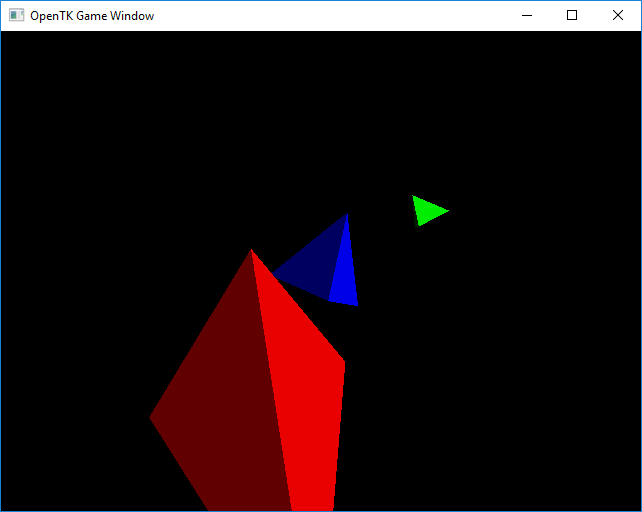
\includegraphics[scale=0.6]{scene.png}
  \caption[Screenshot of example scene of the project]{Project scene}
  \label{fig:exampleScene}
\end{figure}
	
	% Evaluation
	%!TEX root = ../dokumentation.tex

\chapter{Evaluation}\label{cha:Evaluation}

\paragraph{Used example geometry and shaders}

For a basic example a scene consisting out of a tetrahedron which is rendered in three instances is chosen. These instances get different color and different transformations as shown in  \autoref{fig:exampleScene}.

The example for a vertex shader is applying the instance transformation to the vertex position and to its normal, applying a camera transformation to the resulting position and passing through the instance color.

The example for the fragment shader receives the position, the normal and the instance color and applies a light calculation based on a given directional light and the camera position.

\begin{figure}[h!]
  \centering 
  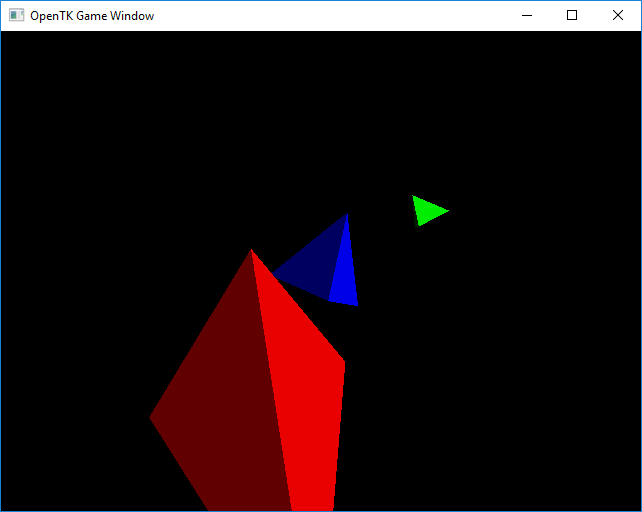
\includegraphics[scale=0.6]{scene.png}
  \caption[Screenshot of example scene of the project]{Project scene}
  \label{fig:exampleScene}
\end{figure}
	
	% Fazit
	%!TEX root = ../dokumentation.tex

\chapter{Conclusion}\label{cha:Conclusion}

As shown in \autoref{cha:Evaluation} it is possible to enable debugging of shaders in the graphics pipeline by simulating them on the CPU. All objectives enumerated in \autoref{paragraph:objective} are met:

\begin{itemize}
\item The different tools VisualStudio provides to aid in the debugging process can be utilized for the shader code written in C\#. Thereby a large number of tools to assist debugging are usable.
\item No specific graphics card or drivers are needed for this method. 
\item It can be switched between a mode where debugging is enabled and a mode where the full performance of the GPU is utilized.
\item The render result per iteration does not have any noticeable differences.
\item Calculating the full graphics pipeline with the shaders in the given example takes about 1.5 seconds per iteration. Consequently all desired debug points occurring in a frame can be reached within this time. This performance is acceptable for a user interface as stated in \autoref{paragraph:objective}.
\end{itemize}

The project implemented as part of this research is limited in its functionality, but it serves as proof for the practicability of the presented methods. It is a functioning method which could be refined and realized in a full tool supporting different source and output languages.

\paragraph{Possible modifications and improvements}

As stated in \autoref{cha:Evaluation} the biggest issue with simulating the graphics pipeline is the performance. This could be improved through multiple ways. The program could be implemented using multiple threads and thereby being able to calculate the simulated steps more parallel on the CPU. Even more improvement would be achieved by implementing parts of the simulated pipeline as compute shaders and running them optimized on the GPU again. For example the performance of the rasterisation process would benefit from this.

To get to the points in the shader faster where it is desired to be able to debug it would also be possible to limit the functionality of the simulated pipeline to this specific part. If for example within the pipeline only the fragments resulting in a specific pixel of the output would be calculated the rest of the rasterisation step could be omitted resulting in far less calculation and time before the desired point to start debugging is reached. The output image of the pipeline would no longer be similar to the resulting image of the shader running on the GPU but the values for this pixel would still be calculated correctly.

It would also be possible to just implement parts of the pipeline. For example it would be possible to debug only a fragment shader. The input values for this shader could be generated without calculating the vertex data. A way to generate these inputs would be to simply give the fragments an input depending on the position of the fragment within the output raster.





	% Inhalt
	%\foreach \i in {01,02,03,04,05,06,07,08,09,...,99} {%
	%	\edef\FileName{content/\i kapitel}%
	%		\IfFileExists{\FileName}{%
	%			\input{\FileName}
	%		}
	%		{%
	%			%file does not exist
	%		}
	%}

	\clearpage
		
	\pagenumbering{roman}
	
%	\renewcommand\bibname{Literaturverzeichnis}
%	\printbibliography

%	\newpage\null\thispagestyle{plain}\newpage
	
	% Glossar
	%\printglossary[style=altlist,title=\langglossar]
	
	% Abkürzungsverzeichnis
	%\clearpage
	%!TEX root = ../dokumentation.tex

\addchap{\langabkverz}
%nur verwendete Akronyme werden letztlich im Abkürzungsverzeichnis des Dokuments angezeigt
%Verwendung: 
%		\ac{Abk.}   --> fügt die Abkürzung ein, beim ersten Aufruf wird zusätzlich automatisch die ausgeschriebene Version davor eingefügt bzw. in einer Fußnote (hierfür muss in header.tex \usepackage[printonlyused,footnote]{acronym} stehen) dargestellt
%		\acs{Abk.}   -->  fügt die Abkürzung ein
%		\acf{Abk.}   --> fügt die Abkürzung UND die Erklärung ein
%		\acl{Abk.}   --> fügt nur die Erklärung ein
%		\acp{Abk.}  --> gibt Plural aus (angefügtes 's'); das zusätzliche 'p' funktioniert auch bei obigen Befehlen
%	siehe auch: http://golatex.de/wiki/%5Cacronym
%	
\begin{acronym}[YTMMM]
\setlength{\itemsep}{-\parsep}

\acro{API}{Application Programming Interface}
\acro{BDSG}{Bundesdatenschutzgesetz}
\acro{CEP}{Complex Event Processing}
\acro{DEA}{Deterministischer endlicher Automat}
\acrodefplural{DEA}[DEAs]{Deterministische endliche Automaten}
\acro{EDA}{Event Driven Architecture}
\acro{GB}{Gigabyte}
\acro{GFS}{Google File System}
\acro{HDFS}{Hadoop Distributed File System}
\acro{HTTP}{Hypertext Transfer Protocol}
\acro{IDE}{Integrated Development Environment}
\acro{IP}{Internetprotokoll}
\acro{KB}{Kilobyte}
\acro{LTS}{Long Term Support}
\acro{MB}{Megabyte}
\acro{MPI}{Message Passing Interface}
\acro{MRC}{Map Reduce Class}
\acro{NAS}{Network Attached Storage}
\acro{NEA}{Nichtdeterministischer endlicher Automat}
\acrodefplural{NEA}[NEAs]{Nichtdeterministische endliche Automaten}
\acro{NFS}{Network File System}
\acro{OS}{Operating System}
\acro{OSDI}{Operating Systems Design and Implementations}
\acro{PAP}{Programmablaufplan}
\acro{PDF}{Portable Document Format}
\acro{POM}{Project Object Model}
\acro{RFC}{Request for Comments}
\acro{RSA}{Rivest, Shamir und Adleman}
\acro{SAN}{Storage Attached Network}
\acro{SPOF}{Single Point of Failure}
\acro{SSH}{Secure Shell}
\acro{TMG}{Telemediengesetz}
\acro{VM}{Virtuelle Maschine}

\end{acronym}


	% Abbildungsverzeichnis
	\cleardoublepage
	\listoffigures
	
%	\newpage\null\thispagestyle{plain}\newpage

	%Tabellenverzeichnis
	%\cleardoublepage
	%\listoftables
	
%	\newpage\null\thispagestyle{plain}\newpage

	% Quellcodeverzeichnis
	\cleardoublepage
	%\lstlistoflistings
	\cleardoublepage

	% Literaturverzeichnis
	\cleardoublepage%
	\printbibliography
	
	% sonstiger Anhang
	\clearpage
	\appendix
	% !TeX root = ../dokumentation.tex

\addchap{\langanhang}

{\Large
	DVD containing the project
}
\pagebreak

	
\end{document}
